\PassOptionsToPackage{unicode=true}{hyperref} % options for packages loaded elsewhere
\PassOptionsToPackage{hyphens}{url}
%
\documentclass[ignorenonframetext,]{beamer}
\usepackage{pgfpages}
\setbeamertemplate{caption}[numbered]
\setbeamertemplate{caption label separator}{: }
\setbeamercolor{caption name}{fg=normal text.fg}
\beamertemplatenavigationsymbolsempty
\usepackage{lmodern}
\usepackage{amssymb,amsmath}
\usepackage{ifxetex,ifluatex}
\usepackage{fixltx2e} % provides \textsubscript
\ifnum 0\ifxetex 1\fi\ifluatex 1\fi=0 % if pdftex
  \usepackage[T1]{fontenc}
  \usepackage[utf8]{inputenc}
  \usepackage{textcomp} % provides euro and other symbols
\else % if luatex or xelatex
  \usepackage{unicode-math}
  \defaultfontfeatures{Ligatures=TeX,Scale=MatchLowercase}
\fi
\usetheme[]{CambridgeUS}
\usecolortheme{beaver}
\usefonttheme{structurebold}
% use upquote if available, for straight quotes in verbatim environments
\IfFileExists{upquote.sty}{\usepackage{upquote}}{}
% use microtype if available
\IfFileExists{microtype.sty}{%
\usepackage[]{microtype}
\UseMicrotypeSet[protrusion]{basicmath} % disable protrusion for tt fonts
}{}
\IfFileExists{parskip.sty}{%
\usepackage{parskip}
}{% else
\setlength{\parindent}{0pt}
\setlength{\parskip}{6pt plus 2pt minus 1pt}
}
\usepackage{hyperref}
\hypersetup{
            pdftitle={A1 - Einleitung und Motivation},
            pdfauthor={Jan-Philipp Kolb},
            pdfborder={0 0 0},
            breaklinks=true}
\urlstyle{same}  % don't use monospace font for urls
\newif\ifbibliography
\usepackage{color}
\usepackage{fancyvrb}
\newcommand{\VerbBar}{|}
\newcommand{\VERB}{\Verb[commandchars=\\\{\}]}
\DefineVerbatimEnvironment{Highlighting}{Verbatim}{commandchars=\\\{\}}
% Add ',fontsize=\small' for more characters per line
\usepackage{framed}
\definecolor{shadecolor}{RGB}{42,33,28}
\newenvironment{Shaded}{\begin{snugshade}}{\end{snugshade}}
\newcommand{\AlertTok}[1]{\textcolor[rgb]{1.00,1.00,0.00}{#1}}
\newcommand{\AnnotationTok}[1]{\textcolor[rgb]{0.00,0.40,1.00}{\textbf{\textit{#1}}}}
\newcommand{\AttributeTok}[1]{\textcolor[rgb]{0.74,0.68,0.62}{#1}}
\newcommand{\BaseNTok}[1]{\textcolor[rgb]{0.27,0.67,0.26}{#1}}
\newcommand{\BuiltInTok}[1]{\textcolor[rgb]{0.74,0.68,0.62}{#1}}
\newcommand{\CharTok}[1]{\textcolor[rgb]{0.02,0.61,0.04}{#1}}
\newcommand{\CommentTok}[1]{\textcolor[rgb]{0.00,0.40,1.00}{\textbf{\textit{#1}}}}
\newcommand{\CommentVarTok}[1]{\textcolor[rgb]{0.74,0.68,0.62}{#1}}
\newcommand{\ConstantTok}[1]{\textcolor[rgb]{0.74,0.68,0.62}{#1}}
\newcommand{\ControlFlowTok}[1]{\textcolor[rgb]{0.26,0.66,0.93}{\textbf{#1}}}
\newcommand{\DataTypeTok}[1]{\textcolor[rgb]{0.74,0.68,0.62}{\underline{#1}}}
\newcommand{\DecValTok}[1]{\textcolor[rgb]{0.27,0.67,0.26}{#1}}
\newcommand{\DocumentationTok}[1]{\textcolor[rgb]{0.00,0.40,1.00}{\textit{#1}}}
\newcommand{\ErrorTok}[1]{\textcolor[rgb]{1.00,1.00,0.00}{\textbf{#1}}}
\newcommand{\ExtensionTok}[1]{\textcolor[rgb]{0.74,0.68,0.62}{#1}}
\newcommand{\FloatTok}[1]{\textcolor[rgb]{0.27,0.67,0.26}{#1}}
\newcommand{\FunctionTok}[1]{\textcolor[rgb]{1.00,0.58,0.35}{\textbf{#1}}}
\newcommand{\ImportTok}[1]{\textcolor[rgb]{0.74,0.68,0.62}{#1}}
\newcommand{\InformationTok}[1]{\textcolor[rgb]{0.00,0.40,1.00}{\textbf{\textit{#1}}}}
\newcommand{\KeywordTok}[1]{\textcolor[rgb]{0.26,0.66,0.93}{\textbf{#1}}}
\newcommand{\NormalTok}[1]{\textcolor[rgb]{0.74,0.68,0.62}{#1}}
\newcommand{\OperatorTok}[1]{\textcolor[rgb]{0.74,0.68,0.62}{#1}}
\newcommand{\OtherTok}[1]{\textcolor[rgb]{0.74,0.68,0.62}{#1}}
\newcommand{\PreprocessorTok}[1]{\textcolor[rgb]{0.74,0.68,0.62}{\textbf{#1}}}
\newcommand{\RegionMarkerTok}[1]{\textcolor[rgb]{0.74,0.68,0.62}{#1}}
\newcommand{\SpecialCharTok}[1]{\textcolor[rgb]{0.02,0.61,0.04}{#1}}
\newcommand{\SpecialStringTok}[1]{\textcolor[rgb]{0.02,0.61,0.04}{#1}}
\newcommand{\StringTok}[1]{\textcolor[rgb]{0.02,0.61,0.04}{#1}}
\newcommand{\VariableTok}[1]{\textcolor[rgb]{0.74,0.68,0.62}{#1}}
\newcommand{\VerbatimStringTok}[1]{\textcolor[rgb]{0.02,0.61,0.04}{#1}}
\newcommand{\WarningTok}[1]{\textcolor[rgb]{1.00,1.00,0.00}{\textbf{#1}}}
\usepackage{graphicx,grffile}
\makeatletter
\def\maxwidth{\ifdim\Gin@nat@width>\linewidth\linewidth\else\Gin@nat@width\fi}
\def\maxheight{\ifdim\Gin@nat@height>\textheight\textheight\else\Gin@nat@height\fi}
\makeatother
% Scale images if necessary, so that they will not overflow the page
% margins by default, and it is still possible to overwrite the defaults
% using explicit options in \includegraphics[width, height, ...]{}
\setkeys{Gin}{width=\maxwidth,height=\maxheight,keepaspectratio}
% Prevent slide breaks in the middle of a paragraph:
\widowpenalties 1 10000
\raggedbottom
\setbeamertemplate{part page}{
\centering
\begin{beamercolorbox}[sep=16pt,center]{part title}
  \usebeamerfont{part title}\insertpart\par
\end{beamercolorbox}
}
\setbeamertemplate{section page}{
\centering
\begin{beamercolorbox}[sep=12pt,center]{part title}
  \usebeamerfont{section title}\insertsection\par
\end{beamercolorbox}
}
\setbeamertemplate{subsection page}{
\centering
\begin{beamercolorbox}[sep=8pt,center]{part title}
  \usebeamerfont{subsection title}\insertsubsection\par
\end{beamercolorbox}
}
\AtBeginPart{
  \frame{\partpage}
}
\AtBeginSection{
  \ifbibliography
  \else
    \frame{\sectionpage}
  \fi
}
\AtBeginSubsection{
  \frame{\subsectionpage}
}
\setlength{\emergencystretch}{3em}  % prevent overfull lines
\providecommand{\tightlist}{%
  \setlength{\itemsep}{0pt}\setlength{\parskip}{0pt}}
\setcounter{secnumdepth}{0}

% set default figure placement to htbp
\makeatletter
\def\fps@figure{htbp}
\makeatother


\title{A1 - Einleitung und Motivation}
\author{Jan-Philipp Kolb}
\date{22 Oktober 2018}

\begin{document}
\frame{\titlepage}

\begin{frame}{Kleine Vorstellungsrunde}
\protect\hypertarget{kleine-vorstellungsrunde}{}

\begin{itemize}
\tightlist
\item
  Wo kommt Ihr her?
\item
  Wo arbeitet oder studiert Ihr?
\item
  Wie beurteilt Ihr Eure Fähigkeiten mit R?
\item
  Habt Ihr Erfahrungen mit anderen Programmiersprachen /
  Statistiksoftware? Wenn ja welche?
\item
  Was sind Eure Erwartungen für diesen Kurs?
\end{itemize}

\end{frame}

\begin{frame}{Informationen vorab}
\protect\hypertarget{informationen-vorab}{}

Normalerweise gibt es große Unterschiede bei Vorkenntnissen und
Fähigkeiten, insbesondere bei diesem Kurs.

\begin{itemize}
\tightlist
\item
  Bitte gebt Bescheid, wenn es zu schnell oder zu langsam geht oder
  etwas unklar geblieben ist.
\item
  Wenn es Fragen gibt - immer fragen
\item
  Wenn Ihr etwas hinzuzufügen habt - sehr gerne
\item
  In diesem Kurs gibt es viele
  \href{http://web.math.ku.dk/~helle/R-intro/exercises.pdf}{\textbf{Übungen}},
  denn das Programmieren / die Nutzung von Geodaten in R lernt man am
  Ende (wie vieles) nur allein.
\item
  Ich habe viele \href{https://www.showmeshiny.com/}{\textbf{Beispiele}}
  - probiert sie aus
\item
  R macht mehr Spaß zusammen - arbeitet zusammen!
\end{itemize}

\end{frame}

\begin{frame}{Disclaimer}
\protect\hypertarget{disclaimer}{}

\begin{itemize}
\tightlist
\item
  Zum Import, zur Verarbeitung und Visualisierung gibt es bereits sehr
  viele Pakete.
\item
  Das Gebiet entwickelt sich sehr schnell.
\item
  Es ist nicht möglich alles davon in diesem Kurs vorzustellen.
\item
  Ich möchte anhand einiger interessanter Beispiele einen Einblick darin
  geben, was alles möglich ist.
\end{itemize}

\end{frame}

\begin{frame}{\href{http://de.slideshare.net/rheimann04/big-social-data-the-spatial-turn-in-big-data}{Laws
of Spatial Sience}}
\protect\hypertarget{laws-of-spatial-sience}{}

\begin{block}{\href{https://en.wikipedia.org/wiki/Tobler's_first_law_of_geography}{Tobler's
law}}

\begin{quote}
everything is related to everything else, but near things are more
related than distant things.
\end{quote}

\end{block}

\begin{block}{\href{https://de.wikipedia.org/wiki/Spatial_turn}{Spatial
Turn}}

\begin{quote}
Spatial turn is a term used to describe an intellectual movement that
places emphasis on place and space in social science and the humanities.
\end{quote}

\end{block}

\end{frame}

\begin{frame}{Motivation -
\href{http://www.spiegel.de/wissenschaft/mensch/deutschland-das-sind-die-groessten-klimasuender-a-1178207.html}{Deutschlands
größte Klimasünder}}
\protect\hypertarget{motivation---deutschlands-grote-klimasunder}{}

\begin{itemize}
\tightlist
\item
  Spiegel Artikel am 16.11.2017 aus Anlass der Jamaika Gespräche
\end{itemize}

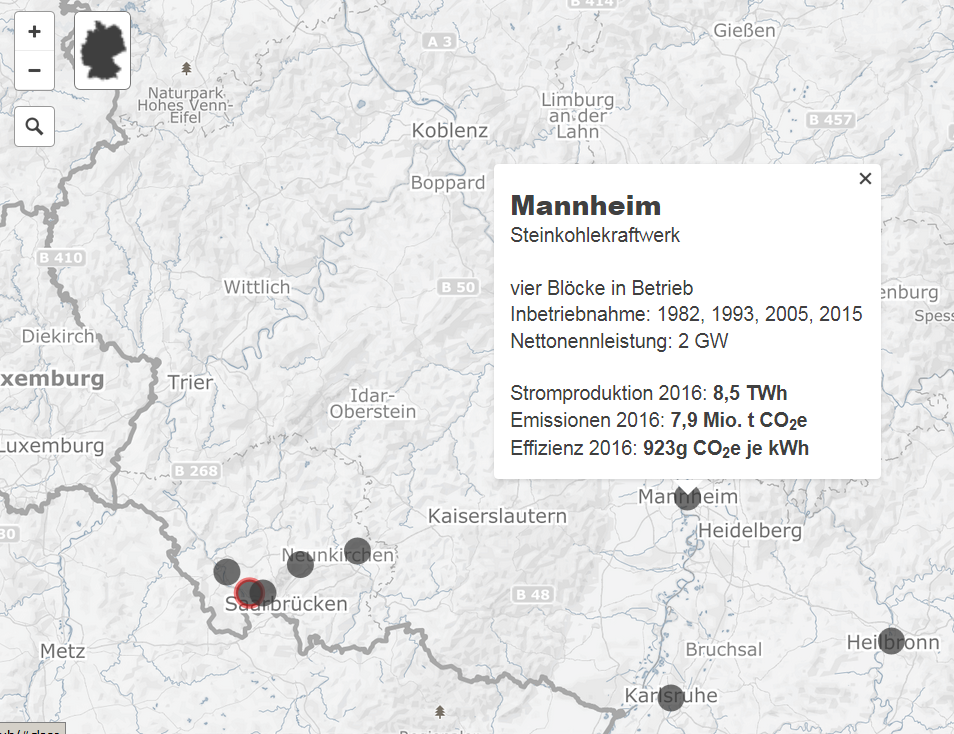
\includegraphics{figure/Kohle_mannheim.PNG}

\end{frame}

\begin{frame}{Motivation}
\protect\hypertarget{motivation}{}

\begin{block}{Motivation allgemein}

\begin{itemize}
\tightlist
\item
  Raumbezug herstellen/nutzen
\item
  Sekundäranalyse für bestehenden Daten
\item
  Analysepotentiale der Geokodierung vorstellen
\item
  Verbindung von sozial- mit raumwissenschaftlichen Daten
\end{itemize}

\end{block}

\begin{block}{Warum die Darstellung in Karten}

\begin{itemize}
\item
  Darstellung in Karten ermöglicht besseres Verständnis von
  sozialwissenschaftlicher Phänomene - Attraktiver Output
\item
  Durch die INSPIRE Richtlinie und \emph{Collaborative Mapping} wächst
  der verfügbare Bestand an Geodaten.
\item
  Daten sind oft frei verfügbar im Internet (z.B. Nutzung von APIs)
\item
  Die Daten sind oft wenig oder gar nicht strukturiert, heterogen und
  oft nicht zur räumlichen Visualisierung vorgesehen, beinhalten aber
  implizit geographische Informationen (Web 2.0)
\item
  Oftmals sind wenig oder keine Metadaten vorhanden
\end{itemize}

\end{block}

\end{frame}

\begin{frame}{Was heißt das für diesen Kurs}
\protect\hypertarget{was-heit-das-fur-diesen-kurs}{}

\begin{block}{Vorgestellt werden:}

\begin{itemize}
\tightlist
\item
  Möglichkeiten für den Download, den Import, die Verarbeitung und die
  Visualisierung von Geodaten
\end{itemize}

\begin{itemize}
\item
  Quellen für Geodaten
\item
  Bspw. die wichtigsten Programmierschnittstellen (APIs) um die Daten zu
  bekommen
\item
  R-Pakete um diese Daten zu verarbeiten und zu visualisieren
\end{itemize}

\end{block}

\end{frame}

\begin{frame}{Das Thema Geodatenlandschaft}
\protect\hypertarget{das-thema-geodatenlandschaft}{}


\includegraphics{figure/BildRatSWDBericht.png}

\end{frame}

\begin{frame}[fragile]{R-Pakete - Zum Download von Geo-Information}
\protect\hypertarget{r-pakete---zum-download-von-geo-information}{}

\begin{block}{\href{https://sites.google.com/site/davidkahle/ggmap}{Das
Paket \texttt{ggmap}}}

\begin{itemize}
\tightlist
\item
  David Kahle and Hadley Wickham: \texttt{ggmap} - Spatial Visualization
  with \texttt{ggplot2}
\end{itemize}

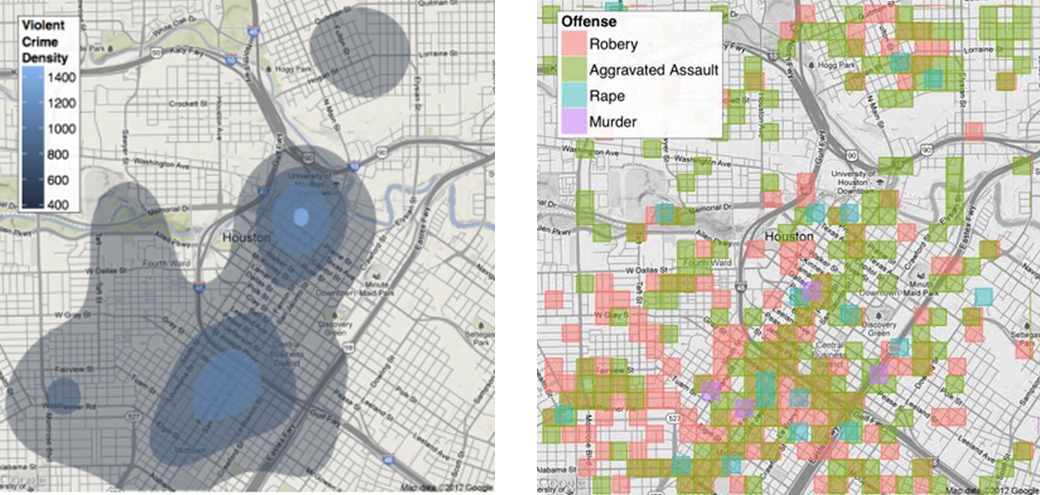
\includegraphics{figure/Rgeopackages.PNG}

\end{block}

\end{frame}

\begin{frame}{\href{http://blog.revolutionanalytics.com/2012/07/making-beautiful-maps-in-r-with-ggmap.html}{Worum
geht es?}}
\protect\hypertarget{worum-geht-es}{}

\begin{block}{Weine probieren im Napa Valley?}

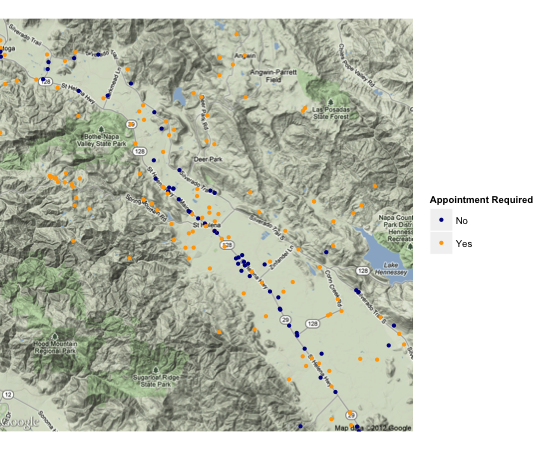
\includegraphics{figure/Wine_nappa.png}

\end{block}

\end{frame}

\begin{frame}{Interessante Visualisierungen -
\href{https://carsten.io/the-racial-dot-map-one-dot-per-person-for-the-entire-u-s/}{One
dot per person}}
\protect\hypertarget{interessante-visualisierungen---one-dot-per-person}{}

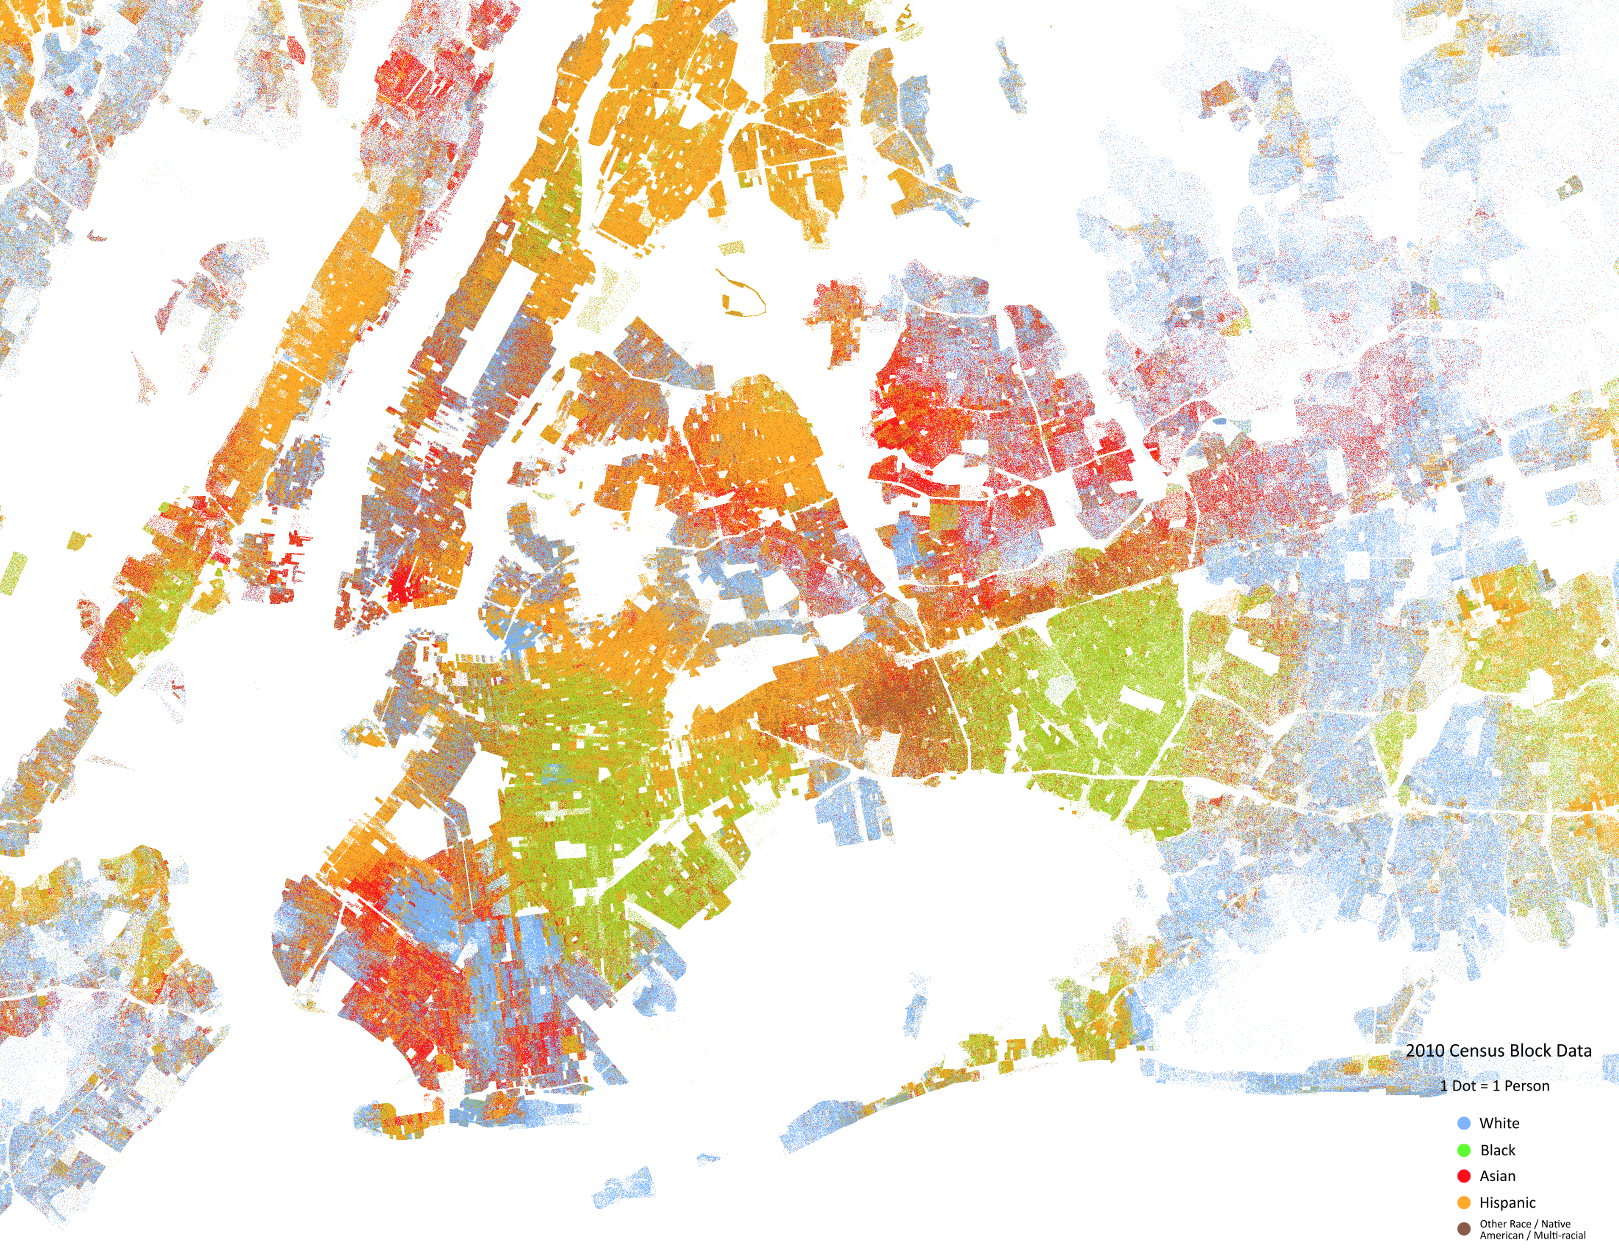
\includegraphics{figure/racemap.png}

\end{frame}

\begin{frame}{Datenquellen}
\protect\hypertarget{datenquellen}{}

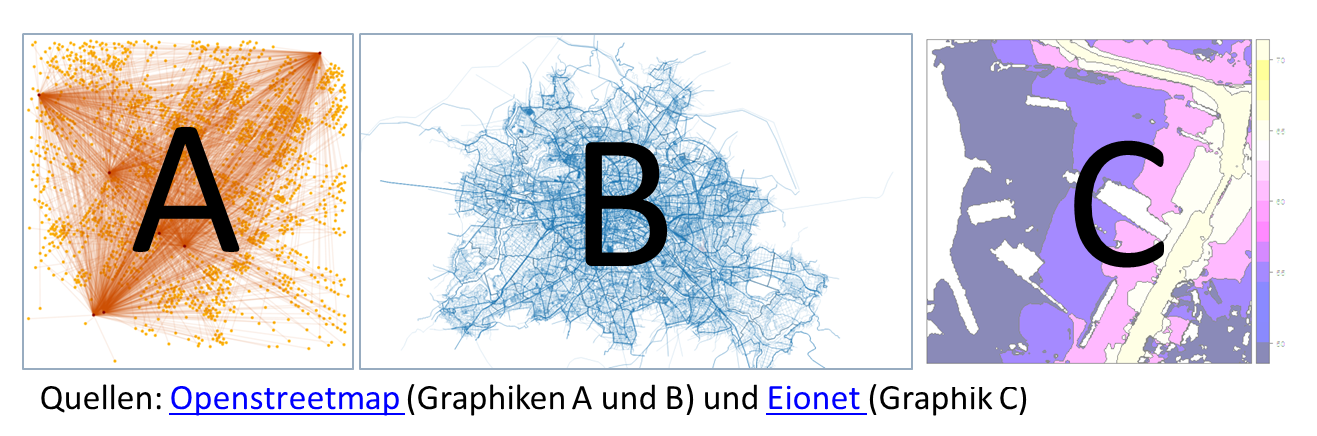
\includegraphics{figure/Datenquellen.png}

\end{frame}

\begin{frame}{Ergebnisse des Zensus 2011 zum
\href{https://www.zensus2011.de/SharedDocs/Aktuelles/Ergebnisse/DemografischeGrunddaten.html?nn=3065474}{\textbf{Download}}}
\protect\hypertarget{ergebnisse-des-zensus-2011-zum-download}{}


\includegraphics{figure/zensus2011_logo.jpg}

\begin{block}{Gemeindeebene}

\begin{itemize}
\tightlist
\item
  Bevölkerung nach Geschlecht, Altersgruppe, Familienstatus,
  Staatsangehörigkeit und Religion
\end{itemize}

\end{block}

\begin{block}{1 \(\text{km}^2\) Raster}

\begin{itemize}
\tightlist
\item
  Bevölkerung, Leerstandsquote, Wohnfläche und Haushaltsgröße
\end{itemize}

\end{block}

\begin{block}{100 \(\text{m}^2\) Raster}

Bevölkerung

\end{block}

\end{frame}

\begin{frame}{Zensus Ergebnisse}
\protect\hypertarget{zensus-ergebnisse}{}

Beispiel Anteil der Personen aus EU27 Land an Einwohnerzahl pro Gemeinde
in Oberfranken

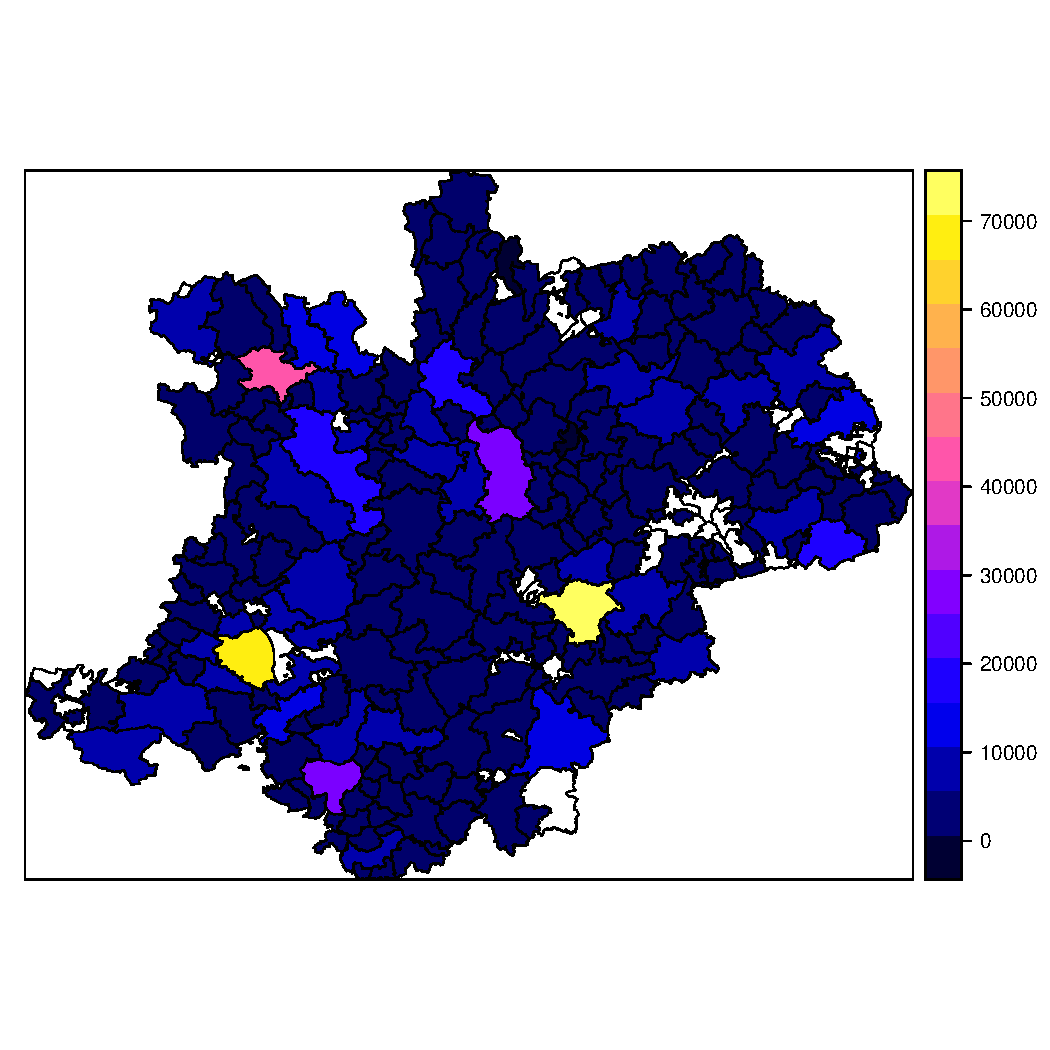
\includegraphics{figure/KRSBamberg_EWZ.pdf}

\end{frame}

\begin{frame}{Zensus Daten zur Leerstandsquote}
\protect\hypertarget{zensus-daten-zur-leerstandsquote}{}

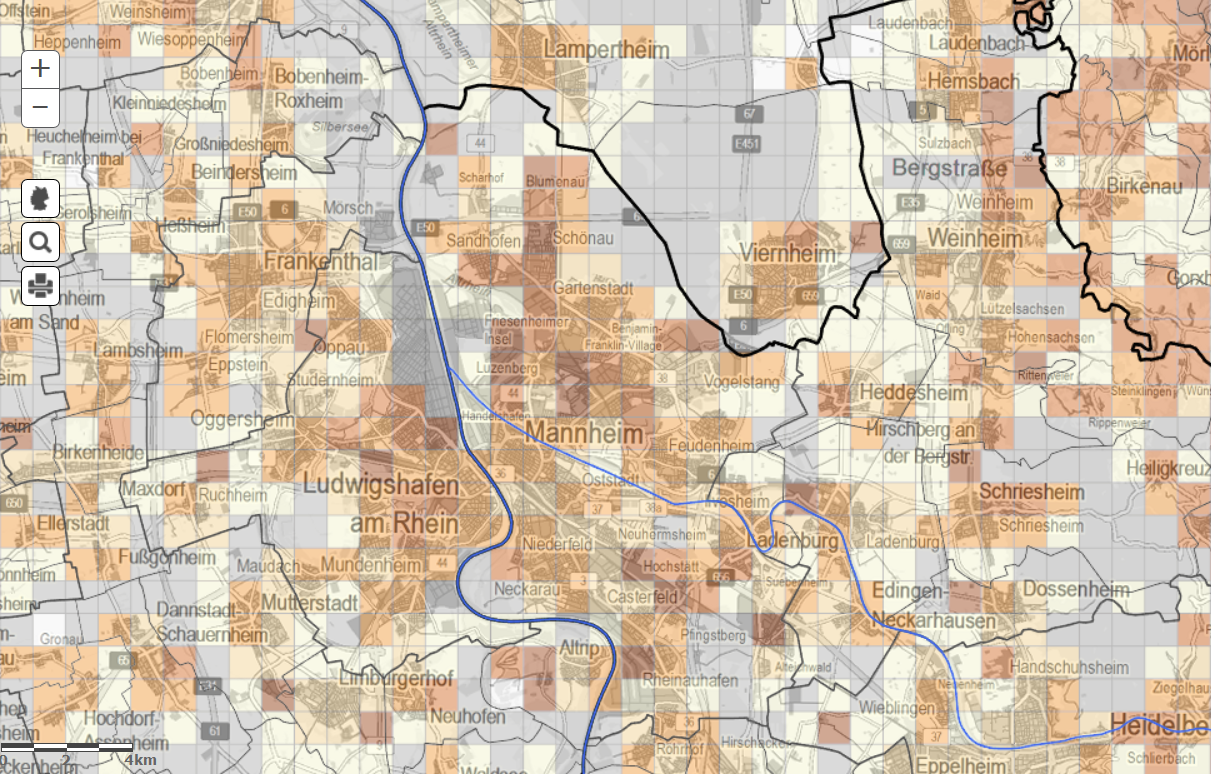
\includegraphics{figure/Leerstandsquote.PNG}

\url{https://atlas.zensus2011.de/}

\end{frame}

\begin{frame}{Datenquelle: Eionet}
\protect\hypertarget{datenquelle-eionet}{}

\begin{block}{\href{http://cdr.eionet.europa.eu/de/eu/noise/df8/colvi7k8q}{Eionet
- Central Data Repository}}

\begin{itemize}
\tightlist
\item
  Europäisches Umweltinformations- und Umweltbeobachtungsnetz
\item
  Qualitätsgesicherte Daten über den Zustand / Einflussfaktoren auf die
  Umwelt in Europa
\item
  Strategische Lärmkartierungen
\end{itemize}

\end{block}

\end{frame}

\begin{frame}{Lärmbelastung durch Schienenlärm}
\protect\hypertarget{larmbelastung-durch-schienenlarm}{}

\begin{block}{Beispiel: Lärmbelastung durch nächtlichen Schienenlärm in
Hamburg}

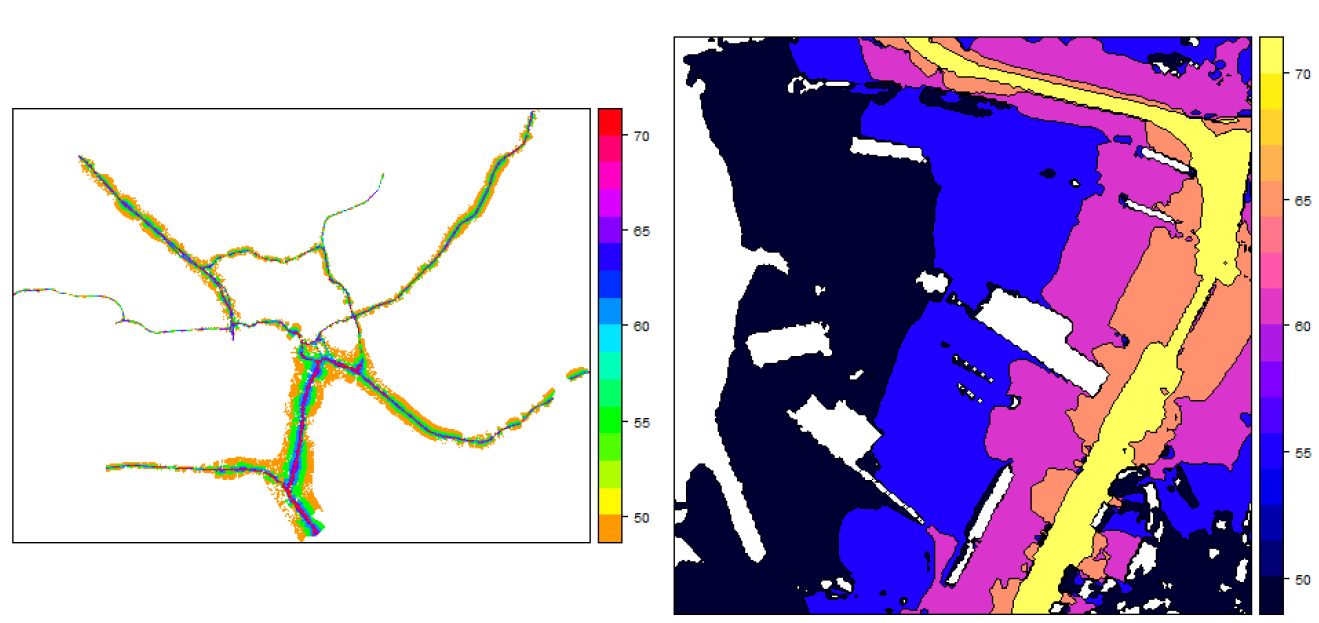
\includegraphics{figure/BSPeionet.PNG}

\end{block}

\end{frame}

\begin{frame}{Institut für ökologische Raumforschung (IÖR)}
\protect\hypertarget{institut-fur-okologische-raumforschung-ior}{}

\begin{block}{IÖR Monitor - Beispiel Siedlungsdichte}

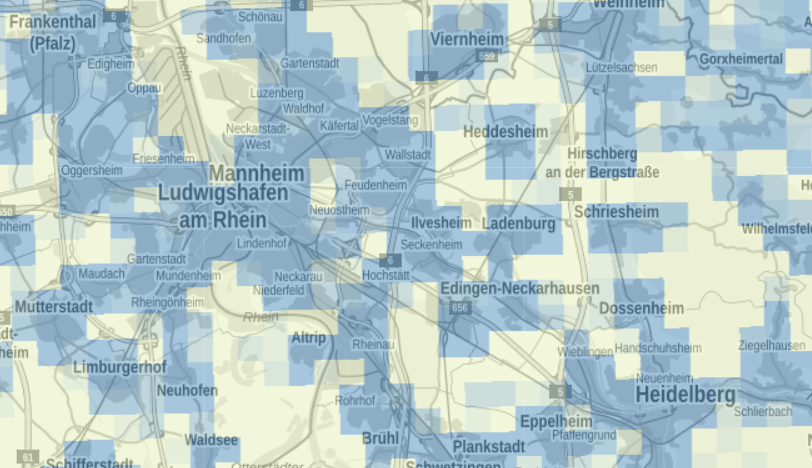
\includegraphics{figure/Siedlungsdichte_ioer.PNG}

\end{block}

\end{frame}

\begin{frame}{Das Openstreetmap Projekt\ldots{}}
\protect\hypertarget{das-openstreetmap-projekt}{}

\begin{block}{Openstreetmap (OSM)}

\begin{itemize}
\tightlist
\item
  Durch kollaboratives Mapping ist eine riesige Datenmenge zugänglich.
\item
  Viele Menschen tragen jeden Tag Informationen bei.
\item
  Die wachsende Menge an Geodaten wird von Freiwilligen gesammelt bzw.
  über Crowdsourcing gewonnen.
\item
  OSM ermöglicht Zugang zu Big Data der Geographie.
\end{itemize}

\end{block}

\end{frame}

\begin{frame}{Drei wichtige OSM Objekttypen}
\protect\hypertarget{drei-wichtige-osm-objekttypen}{}

\begin{block}{Vektordaten werden für den Betrachter dargestellt durch:}

\begin{itemize}
\tightlist
\item
  Polygone sind als (eine Reihe von) verbundenen Prunkten mit gleichem
  Start- und Endpunkt definiert. Die Ausrichtung verläuft gegen den
  Uhrzeigersinn
\end{itemize}

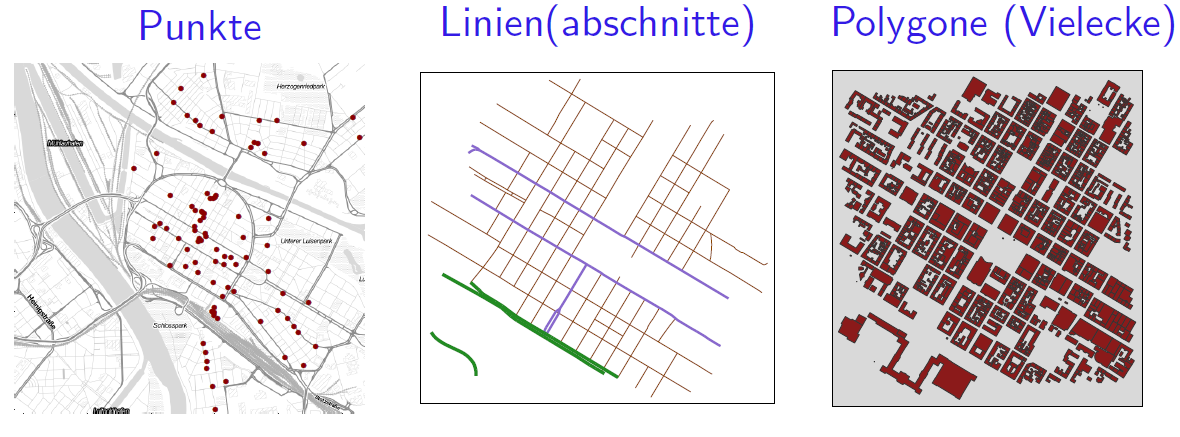
\includegraphics{figure/DreiObjektTypen.PNG}

\end{block}

\end{frame}

\begin{frame}{Beispiel für verfügbare Daten - Straßen in Berlin}
\protect\hypertarget{beispiel-fur-verfugbare-daten---straen-in-berlin}{}

Dargestellt werden OpenStreetMap Daten, die mit der Overpass API
heruntergeladen wurden.

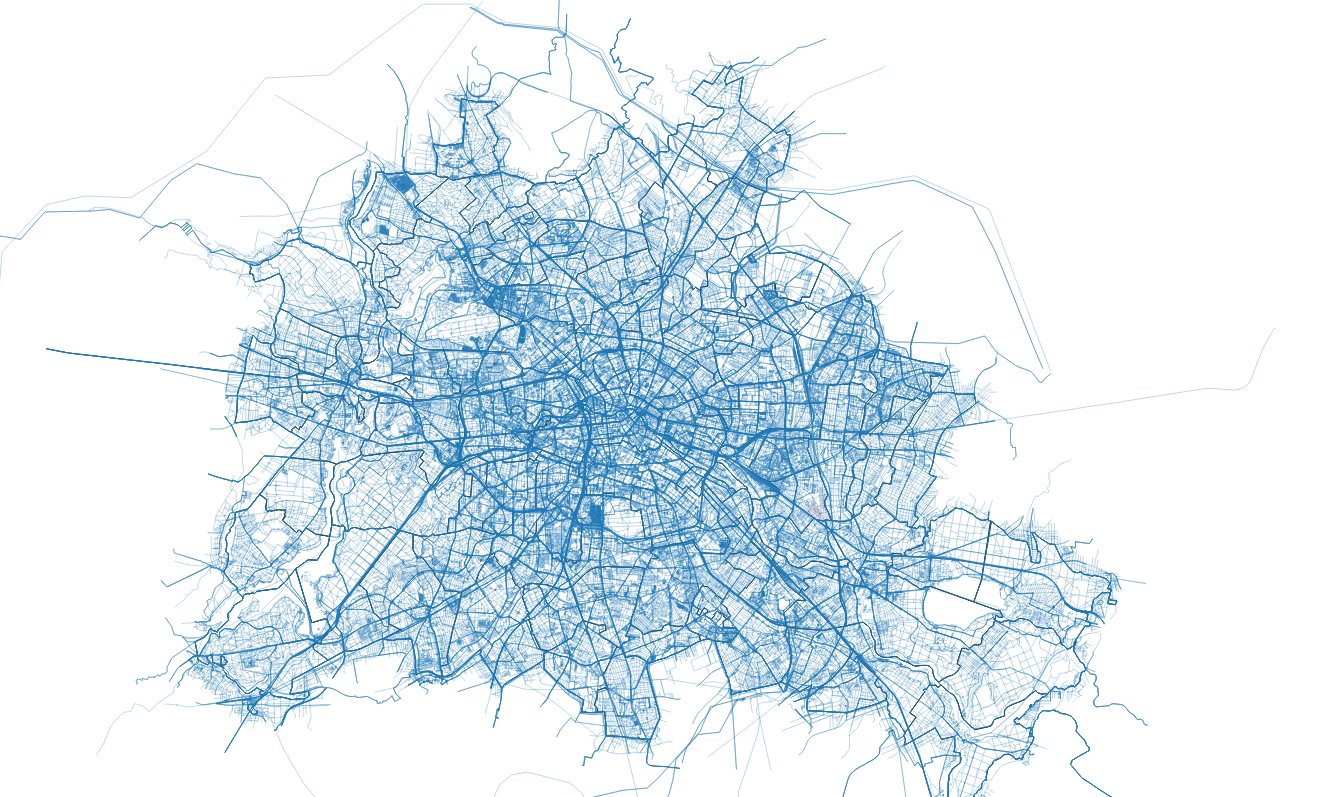
\includegraphics{figure/streets_Berlin2.png}

\end{frame}

\begin{frame}{Paper mit OSM Daten}
\protect\hypertarget{paper-mit-osm-daten}{}

\begin{block}{\href{https://hal.inria.fr/hal-01852585/document}{\textbf{Studie
von Gervasoni et al. (2018)}}}

\begin{itemize}
\tightlist
\item
  Convolutional neural networks for disaggregated population mapping
  using open data
\end{itemize}

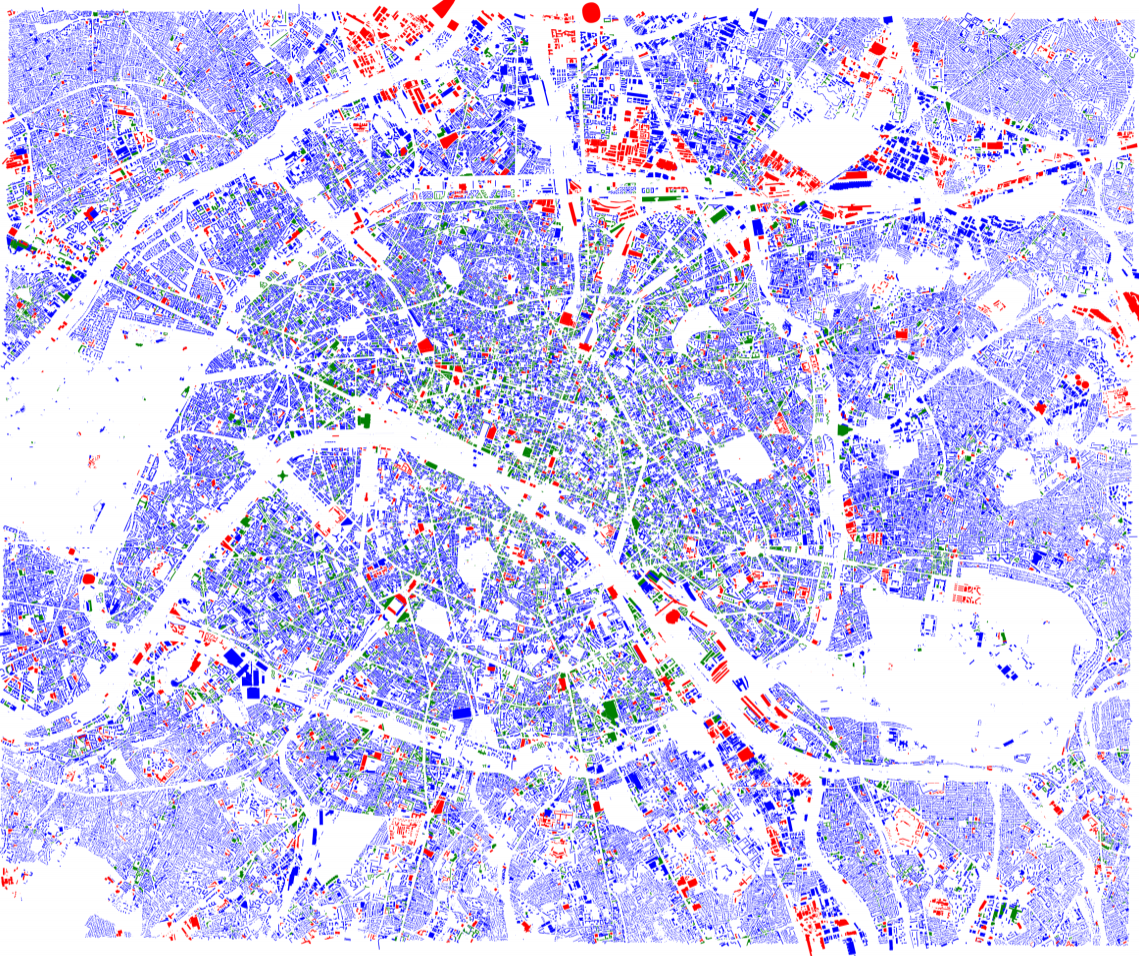
\includegraphics{figure/Buldings_Paris.PNG}

\end{block}

\end{frame}

\begin{frame}{Globale Muster der Straßeninfrastruktur}
\protect\hypertarget{globale-muster-der-straeninfrastruktur}{}

\begin{block}{\href{http://iopscience.iop.org/article/10.1088/1748-9326/aabd42/meta}{\textbf{Studie
von Johan Meijer et al.}}}

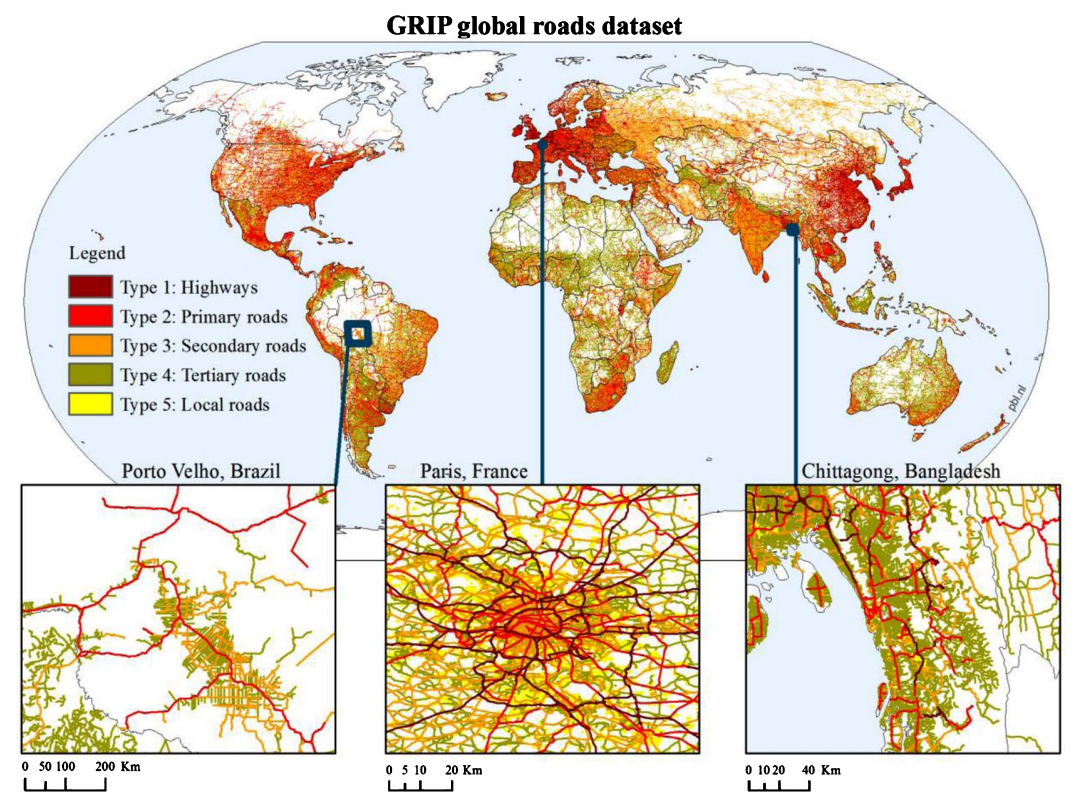
\includegraphics{figure/GRIP_globalroads.PNG}

\end{block}

\end{frame}

\begin{frame}{\href{http://www.visualizing.org/visualizations/mapping-wikipedia-timeline}{Mapping
Wikipedia}}
\protect\hypertarget{mapping-wikipedia}{}

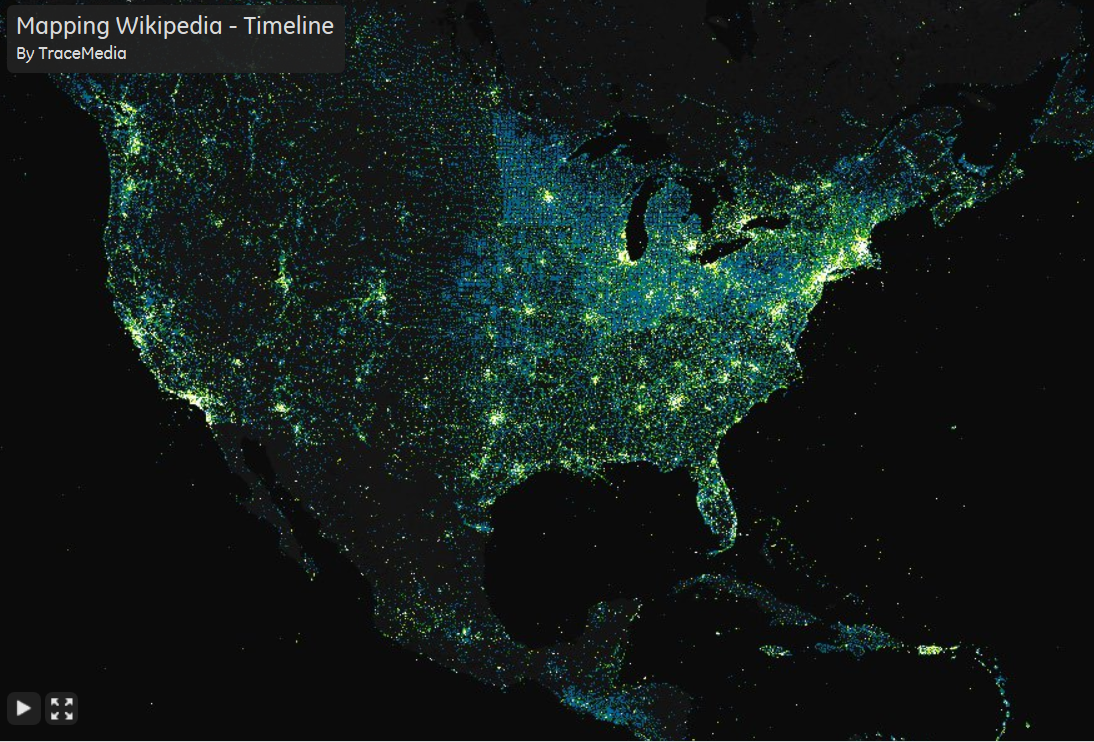
\includegraphics{figure/LuminousUSA.PNG}

\end{frame}

\begin{frame}{\href{http://xkcd.com/1138/}{Allerdings\ldots{}}}
\protect\hypertarget{allerdings}{}

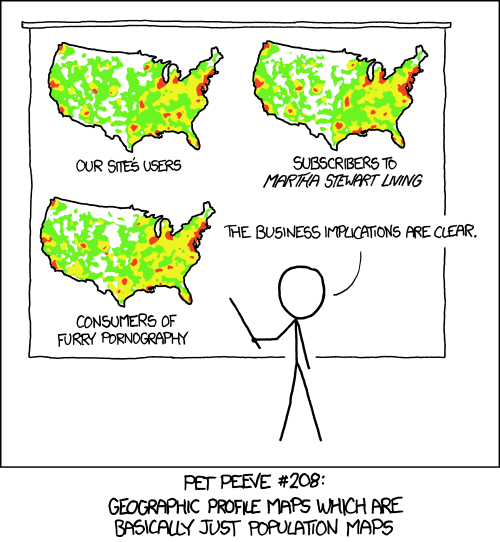
\includegraphics{figure/heatmapComic.png}

\end{frame}

\begin{frame}{Links mit Beispielen}
\protect\hypertarget{links-mit-beispielen}{}

\begin{itemize}
\item
  Shiny App zu
  \href{https://japhilko.shinyapps.io/Choropleths/}{\textbf{Indikatoren}}
  für Europa
\item
  Räumliche Visualisierung in den USA -
  \href{https://rpubs.com/Radcliffe/walmart}{\textbf{Walmarts in den
  USA}}
\item
  \href{http://www.nytimes.com/interactive/2014/09/03/us/the-race-gap-in-americas-police-departments.html?_r=0}{\textbf{Race
  Gap Police USA}} - \href{http://fivethirtyeight.com/}{\textbf{Wahl
  USA}}
\item
  Zeit Artikel zum Zustand der
  \href{http://detektor.fm/digital/datenjournalismus-interaktive-karte-zeigt-marode-deutsche-bahn-bruecken}{\textbf{Eisenbahnbrücken}}
\item
  \href{http://michael-hoerz.de/maps/berlin-bike/}{\textbf{Fahrradunfälle}}
  in Berlin
\item
  \href{http://interaktiv.morgenpost.de/beta-fussballkarte/\#7/51.258/10.756}{\textbf{Verteilung
  Fußballfans}}
\item
  \href{http://news.nationalgeographic.com/news/2014/07/140715-ocean-plastic-debris-trash-pacific-garbage-patch/}{\textbf{Plastiktüten
  im Meer}}
\end{itemize}

\begin{itemize}
\tightlist
\item
  Datensätze zu
  \href{https://www.pegelonline.wsv.de/gast/start}{\textbf{Pegelständen}}
  in Deutschland
\item
  Viele Datensätze auf \href{http://driven-by-data.net/}{\textbf{driven
  by data}}
\end{itemize}

\begin{block}{Resourcen}

\begin{itemize}
\tightlist
\item
  Andreas Plank -
  \href{http://www.chironomidaeproject.com/fileadmin/downloads/Formeln_in_R.pdf}{\textbf{Grafiken
  und Statistik in R}}
\end{itemize}

\end{block}

\end{frame}

\begin{frame}{A1A Übung - zusätzliche Pakete}
\protect\hypertarget{a1a-ubung---zusatzliche-pakete}{}

Gehe auf \url{https://cran.r-project.org/} und suche nach
Paketen\ldots{}

\begin{itemize}
\tightlist
\item
  die Umrisse der Länder der Welt enthalten
\item
  mit denen man die Google maps API nutzen kann
\item
  mit denen man Openstreetmap Daten bekommen kann
\end{itemize}

\end{frame}

\begin{frame}[fragile]{CRAN Task Views}
\protect\hypertarget{cran-task-views}{}

\begin{itemize}
\tightlist
\item
  Bezüglich mancher Themen gibt es einen Überblick über alle wichtigen
  Pakete - (\href{https://cran.r-project.org/web/views/}{\textbf{CRAN
  Task Views}})
\item
  Momentan gibt es 35 Task Views.
\item
  Alle Pakete einer Task-View können mit folgendem
  \href{https://mran.microsoft.com/rpackages/}{\textbf{Befehl}}
  installiert werden:
\end{itemize}

\begin{Shaded}
\begin{Highlighting}[]
\KeywordTok{install.packages}\NormalTok{(}\StringTok{"ctv"}\NormalTok{)}
\KeywordTok{library}\NormalTok{(}\StringTok{"ctv"}\NormalTok{)}
\KeywordTok{install.views}\NormalTok{(}\StringTok{"Spatial"}\NormalTok{)}
\end{Highlighting}
\end{Shaded}

\end{frame}

\end{document}
